\section{Integrales de superficie}

Una integral de superficie acumula una cantidad distribuida sobre una superficie. Si la cantidad es escalar, cada porción aporta el valor del campo multiplicado por su área. Si se integra un campo vectorial orientado, se mide cuánto de ese campo atraviesa la superficie. Ambas construcciones parten del elemento de área $dS$.

\subsection{Integrales de campos escalares sobre gráficas}

Sea $S$ la gráfica $z=f(x,y)$ sobre una región cerrada y acotada $R$ del plano $xy$, con $f$ de clase $C^1$ en un entorno de $R$. Una partición de $R$ determina pequeños parches $S_{ij}$ sobre la superficie. Si $P_{ij}^{*}\in S_{ij}$ y $\Delta S_{ij}$ es el área de ese parche, la suma
\[
\sum_{i,j} g(P_{ij}^{*})\,\Delta S_{ij}
\]
aproxima la acumulación de un campo escalar continuo $g$ sobre $S$. La figura muestra un parche y un punto de muestra; el área que interviene es la del parche curvo, no la de su proyección sobre $R$.

\begingroup\shorthandoff{>}
\begin{center}
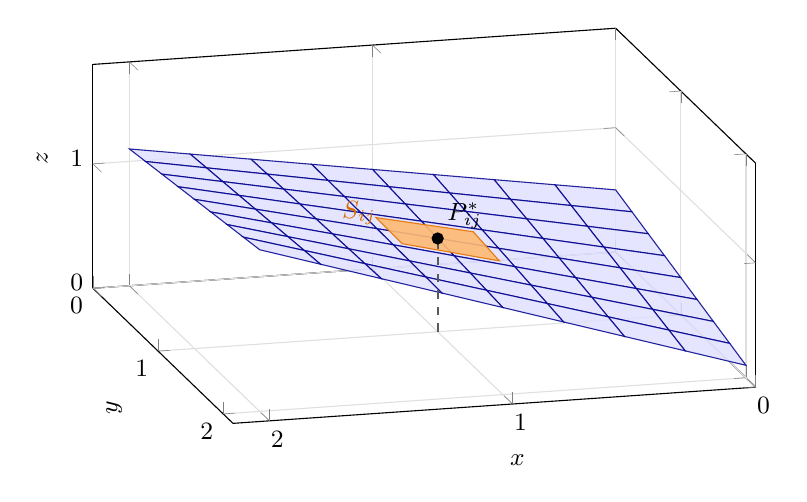
\begin{tikzpicture}
\begin{axis}[width=10cm,height=6.6cm,view={165}{32},axis lines=box,
    xlabel={$x$},ylabel={$y$},zlabel={$z$},
    xmin=0,xmax=2.15,ymin=0,ymax=2.15,zmin=0,zmax=1.8,
    xtick={0,1,2},ytick={0,1,2},ztick={0,1},
    tick label style={font=\small},label style={font=\small},
    grid=major,grid style={gray!25},domain=0:2,y domain=0:2,
    samples=9,samples y=9,z buffer=sort]
\addplot3[surf,shader=flat,draw=blue!55!black,fill=blue!12,opacity=.85]
    {.5+.3*x-.2*y+.15*x*y};
\addplot3[surf,shader=flat,draw=orange!90!black,fill=orange!55,
    opacity=.9,domain=.8:1.2,y domain=.8:1.2,
    samples=2,samples y=2,z buffer=none]
    {.5+.3*x-.2*y+.15*x*y};
\addplot3[gray!70!black,dashed,thick]
    coordinates {(1,1,0) (1,1,.75)};
\addplot3[only marks,mark=*,mark size=2pt,black]
    coordinates {(1,1,.75)};
\node[above right,font=\small] at (axis cs:1,1,.75) {$P_{ij}^{*}$};
\node[font=\small,orange!85!black] at (axis cs:1.35,1.1,1.05) {$S_{ij}$};
\end{axis}
\end{tikzpicture}
\end{center}
\endgroup

\begin{mydefinition}{Integral de superficie de un campo escalar}
Sea $g:S\to\mathbb R$ continua y sea $S$ una superficie suave por partes. La integral de $g$ sobre $S$ se define por el límite de sumas de parches
\[
\iint_S g\,dS
=\lim_{S_{ij}\to0}
\sum_{i,j = (0,0)}^{(\infty,\infty)}g(P_{ij}^{*})\,\Delta S_{ij},
\]
si el límite existe y no depende de la elección de los puntos de muestra.
\end{mydefinition}

Para la gráfica se usa $\vec r(x,y)=\langle x,y,f(x,y)\rangle$. Los vectores tangentes a las curvas coordenadas y su producto cruz son
\[
\vec r_x=\langle1,0,f_x\rangle,
\qquad
\vec r_y=\langle0,1,f_y\rangle,
\qquad
\vec r_x\times\vec r_y=\langle-f_x,-f_y,1\rangle.
\]
Por tanto, un rectángulo de área $\Delta x\,\Delta y$ en $R$ corresponde aproximadamente a un paralelogramo tangente de área $\lVert\vec r_x\times\vec r_y\rVert\Delta x\,\Delta y$.
\begingroup\shorthandoff{>}
\begin{center}
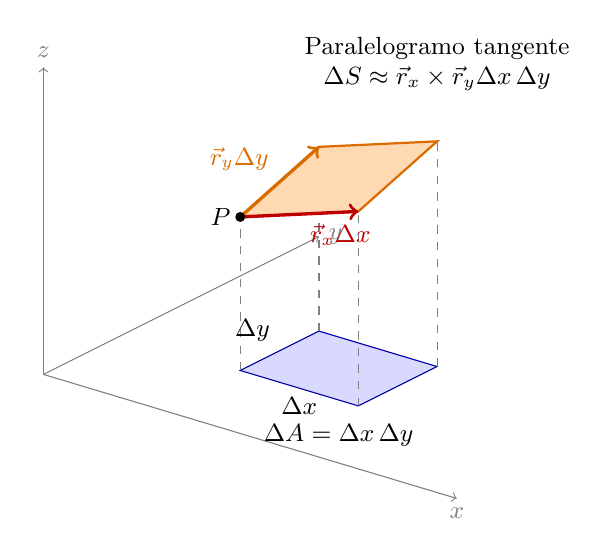
\begin{tikzpicture}[x={(1.5cm,-.45cm)},y={(1cm,.5cm)},
    z={(0cm,1.3cm)},every node/.style={font=\small}]
    \draw[->,gray] (0,0,0)--(3.5,0,0) node[below] {$x$};
    \draw[->,gray] (0,0,0)--(0,3.5,0) node[right] {$y$};
    \draw[->,gray] (0,0,0)--(0,0,3) node[above] {$z$};
    \filldraw[fill=blue!15,draw=blue!65!black]
        (1,1,0)--(2,1,0)--(2,2,0)--(1,2,0)--cycle;
    \draw[gray,dashed] (1,1,0)--(1,1,1.5);
    \draw[gray,dashed] (2,1,0)--(2,1,1.9);
    \draw[gray,dashed] (2,2,0)--(2,2,2.2);
    \draw[gray,dashed] (1,2,0)--(1,2,1.8);
    \filldraw[fill=orange!30,draw=orange!85!black,thick]
        (1,1,1.5)--(2,1,1.9)--(2,2,2.2)--(1,2,1.8)--cycle;
    \draw[->,red!75!black,very thick] (1,1,1.5)--(2,1,1.9)
        node[midway,below right] {$\vec r_x\Delta x$};
    \draw[->,orange!85!black,very thick] (1,1,1.5)--(1,2,1.8)
        node[midway,above left] {$\vec r_y\Delta y$};
    \fill (1,1,1.5) circle (1.8pt) node[left] {$P$};
    \path (1,1,0)--(2,1,0) node[midway,below] {$\Delta x$};
    \path (1,1,0)--(1,2,0) node[midway,above left] {$\Delta y$};
    \node[below] at (1.5,1.5,-.45) {$\Delta A=\Delta x\,\Delta y$};
    \node[above,align=center] at (2,2,2.6)
        {Paralelogramo tangente\\
        $\Delta S\approx\lVert\vec r_x\times\vec r_y\rVert\Delta x\,\Delta y$};
\end{tikzpicture}
\end{center}
\endgroup

Al pasar al límite se obtiene
\begin{mytheorem}{Integral escalar sobre una gráfica}
Si $S:z=f(x,y)$ está situada sobre $R$ y $g$ es continua en $S$, entonces
\[
\iint_S g(x,y,z)\,dS
=\iint_R g\bigl(x,y,f(x,y)\bigr)
\sqrt{1+f_x(x,y)^2+f_y(x,y)^2}\,dA.
\]
\end{mytheorem}

Para evaluar la integral se identifica primero la proyección $R$. Después se sustituye $z=f(x,y)$ en $g$, se calcula el factor $\sqrt{1+f_x^2+f_y^2}$ y se integra sobre $R$.

\paragraph{Ejemplo 1. Campo escalar sobre un plano}
Sea $S:z=1+x+y$ sobre $R=[0,1]\times[0,1]$. Se calcula $\iint_S z\,dS$. Como $f_x=f_y=1$, se tiene $dS=\sqrt3\,dx\,dy$ y, sobre $S$, el integrando $z$ vale $1+x+y$. Así,
\begin{align*}
\iint_S z\,dS
&=\sqrt3\int_0^1\int_0^1(1+x+y)\,dy\,dx\\
&=\sqrt3\int_0^1\left(\frac32+x\right)dx
=2\sqrt3.
\end{align*}
La figura muestra el parche plano y su proyección cuadrada. El valor de $z$ aumenta hacia la esquina elevada, mientras que el factor de área permanece constante.

\begingroup\shorthandoff{>}
\begin{center}
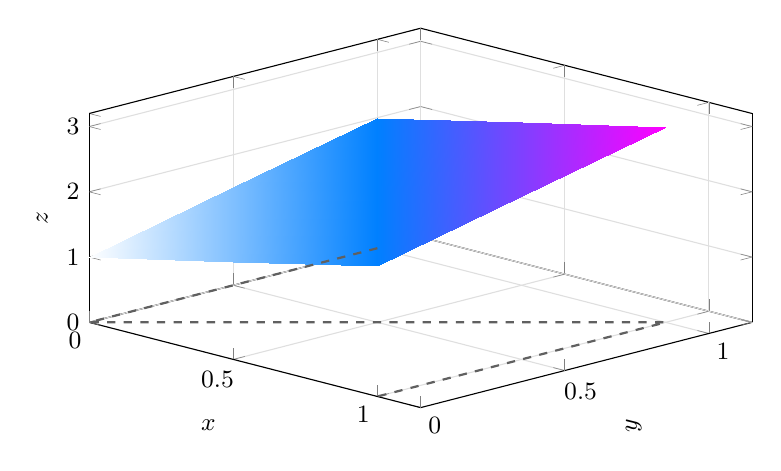
\begin{tikzpicture}
\begin{axis}[width=10cm,height=6.4cm,view={45}{30},axis lines=box,
    xlabel={$x$},ylabel={$y$},zlabel={$z$},
    xmin=0,xmax=1.15,ymin=0,ymax=1.15,zmin=0,zmax=3.2,
    xtick={0,.5,1},ytick={0,.5,1},ztick={0,1,2,3},
    tick label style={font=\small},label style={font=\small},
    grid=major,grid style={gray!25},domain=0:1,y domain=0:1,
    samples=3,samples y=3,z buffer=sort]
\addplot3[surf,shader=interp,colormap/cool]
    {1+x+y};
\addplot3[gray!75!black,dashed,thick]
    coordinates {(0,0,0) (1,0,0) (1,1,0) (0,1,0) (0,0,0)};
\end{axis}
\end{tikzpicture}
\end{center}
\endgroup

\paragraph{Ejemplo 2. Campo escalar sobre un paraboloide}
Sea $S:z=x^2+y^2$ sobre el disco $R:x^2+y^2\leq1$. De nuevo se calcula $\iint_S z\,dS$, pero ahora $f_x=2x$ y $f_y=2y$. Con $x=\rho\cos\theta$, $y=\rho\sin\theta$ y $z=\rho^2$,
\begin{align*}
\iint_S z\,dS
&=\iint_R(x^2+y^2)\sqrt{1+4x^2+4y^2}\,dA\\
&=2\pi\int_0^1\rho^3\sqrt{1+4\rho^2}\,d\rho.
\end{align*}
La sustitución $t=1+4\rho^2$ da $\rho^3\,d\rho=(t-1)\,dt/32$. En consecuencia,
\begin{align*}
\iint_S z\,dS
&=\frac{\pi}{16}\int_1^5(t-1)\sqrt t\,dt\\
&=\frac{\pi}{16}
\left[\frac25t^{5/2}-\frac23t^{3/2}\right]_1^5
=\frac{\pi}{60}(25\sqrt5+1).
\end{align*}

\begingroup\shorthandoff{>}
\begin{center}
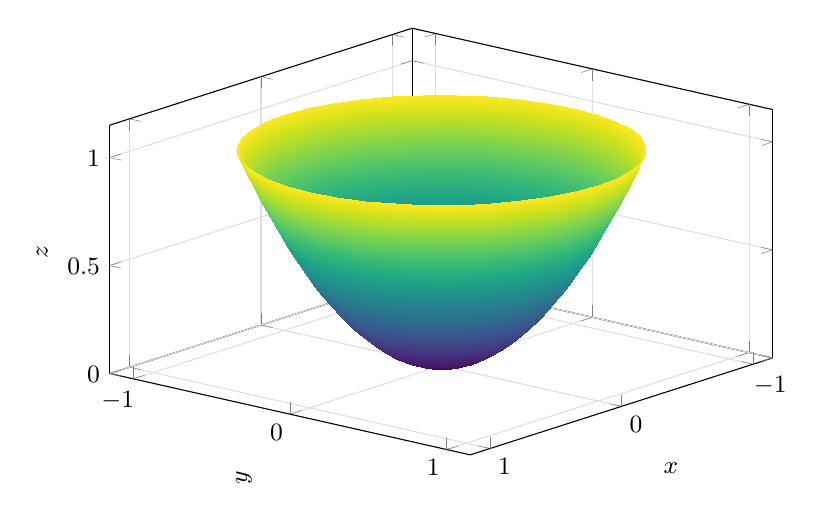
\begin{tikzpicture}
\begin{axis}[width=10cm,height=7cm,view={130}{27},axis lines=box,
    xlabel={$x$},ylabel={$y$},zlabel={$z$},
    xmin=-1.15,xmax=1.15,ymin=-1.15,ymax=1.15,zmin=0,zmax=1.15,
    xtick={-1,0,1},ytick={-1,0,1},ztick={0,.5,1},
    tick label style={font=\small},label style={font=\small},
    grid=major,grid style={gray!25},domain=0:360,y domain=0:1,
    samples=41,samples y=17,z buffer=sort]
\addplot3[surf,shader=interp,colormap/viridis]
    ({y*cos(x)},{y*sin(x)},{y^2});
\end{axis}
\end{tikzpicture}
\end{center}
\endgroup

\subsection{Densidades sobre una superficie}

Si $\sigma(P)$ expresa una cantidad por unidad de área en $P\in S$, entonces $\sigma(P)\,dS$ representa la cantidad contenida aproximadamente en un parche pequeño. La acumulación total es
\[
A=\iint_S\sigma(P)\,dS.
\]
La misma fórmula sirve para distintas magnitudes: si $\sigma$ es densidad superficial de masa, $A$ es la masa de una lámina; si es densidad superficial de carga eléctrica, $A$ es la carga total. 
\paragraph{Ejemplo 3. Masa de un hemisferio}
Sea $S$ el hemisferio superior $z=\sqrt{4-x^2-y^2}$, $x^2+y^2\leq4$, con densidad superficial de masa $\sigma(x,y,z)=kz$, donde $k>0$ tiene las unidades correspondientes. La densidad aumenta con la altura, como sugiere la figura.

En el interior del disco $R:x^2+y^2\leq4$ se tiene
\[
f_x=-\frac{x}{z},\qquad f_y=-\frac{y}{z},\qquad
\sqrt{1+f_x^2+f_y^2}=\frac{2}{z}.
\]
El producto $\sigma\,dS$ se simplifica aunque el factor de área crece al acercarse al borde:
\begin{align*}
M&=\iint_S kz\,dS
=\iint_R kz\,\frac{2}{z}\,dA\\
&=2k\operatorname{area}(R)=8\pi k.
\end{align*}
La igualdad se obtiene integrando primero sobre discos de radio menor que $2$ y tomando el límite.

\begingroup\shorthandoff{>}
\begin{center}
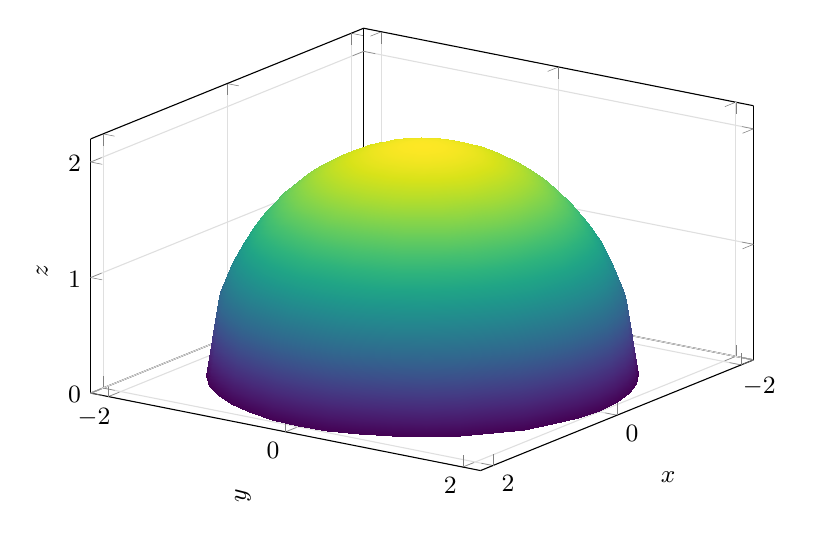
\begin{tikzpicture}
\begin{axis}[width=10cm,height=7.2cm,view={125}{28},axis lines=box,
    xlabel={$x$},ylabel={$y$},zlabel={$z$},
    xmin=-2.2,xmax=2.2,ymin=-2.2,ymax=2.2,zmin=0,zmax=2.2,
    xtick={-2,0,2},ytick={-2,0,2},ztick={0,1,2},
    tick label style={font=\small},label style={font=\small},
    grid=major,grid style={gray!25},domain=0:360,y domain=0:2,
    samples=41,samples y=19,z buffer=sort]
\addplot3[surf,shader=interp,colormap/viridis]
    ({y*cos(x)},{y*sin(x)},{sqrt(4-y^2)});
\end{axis}
\end{tikzpicture}
\end{center}
\endgroup

\subsection{Integrales escalares sobre superficies paramétricas}

Sea $D$ una región cerrada y acotada con frontera suave por partes, y sea $\vec r:D\to\mathbb R^3$ una parametrización de $S$, de clase $C^1$ en un entorno de $D$ y regular en su interior. Se escribe
\[
\vec r(u,v)=\langle x(u,v),y(u,v),z(u,v)\rangle,
\qquad (u,v)\in D.
\]
Los parámetros $u$ y $v$ son las coordenadas de un dominio plano. La parametrización asigna a cada par $(u,v)$ un punto de la superficie en el espacio $xyz$. Así, para integrar sobre $S$ se expresa la posición mediante $u,v$ y se realiza la integral en $D$. En general, $D$ no es la proyección de $S$ sobre el plano $xy$: los parámetros pueden representar, por ejemplo, un ángulo y una altura.

La figura muestra esta correspondencia para una porción del cilindro unitario:
\[
\vec r(u,v)=\langle\cos u,\sin u,v\rangle,
\qquad D=[0,\pi/2]\times[0,2].
\]
Las líneas horizontales del dominio, donde $v$ es constante, se transforman en arcos de circunferencia; las líneas verticales, donde $u$ es constante, se transforman en segmentos verticales. El rectángulo naranja se transforma en un parche curvo.

\begingroup\shorthandoff{>}
\begin{center}
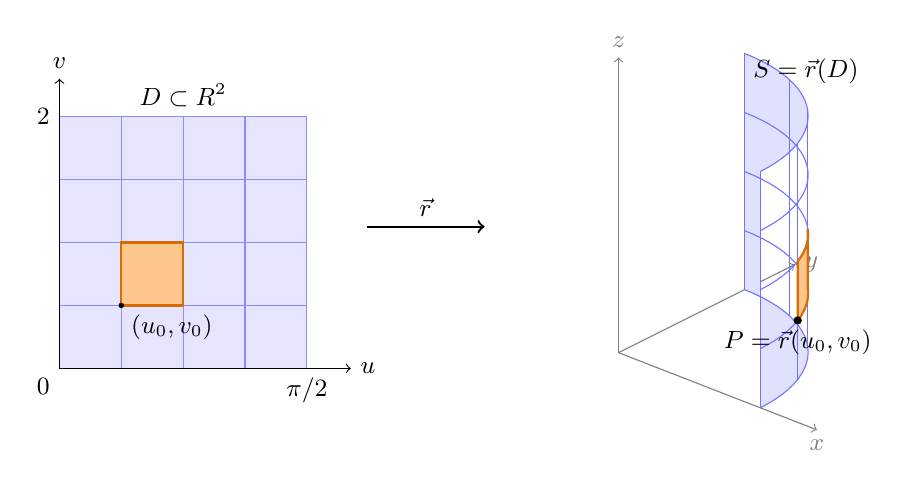
\begin{tikzpicture}[every node/.style={font=\small}]
\begin{scope}[x=2cm,y=1.6cm]
    \fill[blue!10] (0,0) rectangle (1.5708,2);
    \draw[blue!45] (0,0) grid[xstep=.3927,ystep=.5] (1.5708,2);
    \filldraw[fill=orange!45,draw=orange!85!black,thick]
        (.3927,.5) rectangle (.7854,1);
    \draw[->] (0,0)--(1.85,0) node[right] {$u$};
    \draw[->] (0,0)--(0,2.3) node[above] {$v$};
    \node[below left] at (0,0) {$0$};
    \node[below] at (1.5708,0) {$\pi/2$};
    \node[left] at (0,2) {$2$};
    \node[above] at (.7854,2) {$D\subset\mathbb R^2$};
    \fill (.3927,.5) circle (1pt) node[below right] {$(u_0,v_0)$};
\end{scope}
\draw[->,thick] (3.9,1.8)--(5.4,1.8) node[midway,above] {$\vec r$};
\begin{scope}[shift={(7.1,.2)},x={(1.8cm,-.7cm)},
    y={(1.6cm,.8cm)},z={(0cm,1.5cm)}]
    \draw[->,gray] (0,0,0)--(1.4,0,0) node[below] {$x$};
    \draw[->,gray] (0,0,0)--(0,1.4,0) node[right] {$y$};
    \draw[->,gray] (0,0,0)--(0,0,2.5) node[above] {$z$};
    \fill[blue!12] plot[domain=0:90,samples=25] ({cos(\x)},{sin(\x)},0)
        --(0,1,2) --plot[domain=90:0,samples=25] ({cos(\x)},{sin(\x)},2)--cycle;
    \foreach \h in {0,.5,1,1.5,2}
        \draw[blue!55] plot[domain=0:90,samples=25] ({cos(\x)},{sin(\x)},\h);
    \foreach \a in {0,22.5,45,67.5,90}
        \draw[blue!55] ({cos(\a)},{sin(\a)},0)--({cos(\a)},{sin(\a)},2);
    \filldraw[fill=orange!45,draw=orange!85!black,thick]
        plot[domain=22.5:45,samples=12] ({cos(\x)},{sin(\x)},.5)
        --({cos(45)},{sin(45)},1)
        --plot[domain=45:22.5,samples=12] ({cos(\x)},{sin(\x)},1)--cycle;
    \fill ({cos(22.5)},{sin(22.5)},.5) circle (1.5pt)
        node[below] {$P=\vec r(u_0,v_0)$};
    \node[above] at (.7,.7,2.15) {$S=\vec r(D)$};
\end{scope}
\end{tikzpicture}
\end{center}
\endgroup

Al fijar $v=v_0$, la función $u\mapsto\vec r(u,v_0)$ describe una curva sobre $S$ cuyo vector tangente es $\vec r_u$. De manera análoga, al fijar $u=u_0$ se obtiene una curva con vector tangente $\vec r_v$. La regularidad significa que $\vec r_u\times\vec r_v\neq\vec0$; por tanto, estas dos direcciones generan el plano tangente.

Para incrementos positivos pequeños $\Delta u$ y $\Delta v$, la aproximación lineal de cada curva coordenada da
\[
\vec r(u+\Delta u,v)-\vec r(u,v)\approx\vec r_u(u,v)\Delta u,
\qquad
\vec r(u,v+\Delta v)-\vec r(u,v)\approx\vec r_v(u,v)\Delta v.
\]
Ambos vectores se evalúan en el mismo punto $(u,v)$. El parche curvo se aproxima mediante el paralelogramo tangente de lados $\vec r_u\Delta u$ y $\vec r_v\Delta v$, es decir, la norma de su producto cruz:
\[
\Delta S\approx
\bigl\lVert(\vec r_u\Delta u)\times(\vec r_v\Delta v)\bigr\rVert
=\lVert\vec r_u\times\vec r_v\rVert\,\Delta u\,\Delta v.
\]
El factor $\lVert\vec r_u\times\vec r_v\rVert$ convierte el área del dominio de parámetros en área sobre la superficie. Incluye tanto el cambio de longitud en cada dirección como el ángulo entre ellas; por ello, no basta con multiplicar $\lVert\vec r_u\rVert$ y $\lVert\vec r_v\rVert$ si los vectores no son perpendiculares. En notación diferencial se escribe
\[
dS=\lVert\vec r_u\times\vec r_v\rVert\,du\,dv.
\]
En una partición de $D$, un punto de muestra $(u_{ij}^{*},v_{ij}^{*})$ corresponde a $P_{ij}^{*}=\vec r(u_{ij}^{*},v_{ij}^{*})$. Por tanto, la suma de las contribuciones de los parches toma la forma aproximada
\[
\sum_{i,j}g(P_{ij}^{*})\,\Delta S_{ij}
\approx\sum_{i,j}
g\bigl(\vec r(u_{ij}^{*},v_{ij}^{*})\bigr)
\lVert\vec r_u(u_{ij}^{*},v_{ij}^{*})\times
\vec r_v(u_{ij}^{*},v_{ij}^{*})\rVert\,\Delta u_i\,\Delta v_j.
\]
Al refinar la partición, el lado derecho converge a una integral doble sobre $D$. La condición de recorrer la superficie una sola vez evita contar repetidamente el área de un mismo parche.

\begin{mytheorem}{Integral escalar sobre una superficie paramétrica}
Si $\vec r$ recorre $S$ una sola vez salvo, posiblemente, en la frontera de $D$, y $g$ es continua en $S$, entonces
\[
\iint_S g\,dS
=\iint_D g\bigl(\vec r(u,v)\bigr)
\lVert\vec r_u(u,v)\times\vec r_v(u,v)\rVert\,du\,dv.
\]
\end{mytheorem}

Para una gráfica $\vec r(u,v)=\langle u,v,f(u,v)\rangle$, se tiene $\lVert\vec r_u\times\vec r_v\rVert=\sqrt{1+f_u^2+f_v^2}$, de modo que esta expresión recupera la fórmula anterior. La norma del producto cruz hace que la integral escalar no dependa del sentido elegido para recorrer los parámetros.

Si además se realiza un cambio de variables en la proyección $xy$, se escriben $x=x(u,v)$, $y=y(u,v)$ y se parametriza la gráfica mediante
\[
\vec r(u,v)=\langle x(u,v),y(u,v),f(x(u,v),y(u,v))\rangle.
\]
Por ejemplo, para $z=x^2+y^2$ con coordenadas polares en la proyección, se obtiene
\[
x=u\cos v,\qquad y=u\sin v,\qquad
\vec r(u,v)=\langle u\cos v,u\sin v,u^2\rangle.
\]
Aquí $u$ representa la distancia al origen en el plano $xy$ y $v$ el ángulo. En una región que evite el origen y el corte angular, el cambio inverso es $u=\sqrt{x^2+y^2}$ y $v$ es el argumento de $(x,y)$ en el intervalo angular elegido. Así se distingue el cambio de coordenadas entre los planos $xy$ y $uv$ de la parametrización, que lleva el dominio $uv$ a la superficie en $xyz$.

\paragraph{Ejemplo 4. Integral escalar sobre un cilindro}
La superficie lateral de un cilindro de radio $a$ y altura $L$ se parametriza por
\[
\vec r(u,v)=\langle a\cos u,a\sin u,v\rangle,
\qquad0\leq u\leq2\pi,\quad0\leq v\leq L.
\]
Como $\lVert\vec r_u\times\vec r_v\rVert=a$, la integral del campo escalar $g(x,y,z)=z$ es
\[
\iint_S z\,dS
=\int_0^{2\pi}\int_0^L av\,dv\,du
=\pi aL^2.
\]
Cada franja horizontal tiene la misma circunferencia, pero el valor de $z$ aumenta con la altura.
La figura muestra el caso $a=1$ y $L=2$. El parche naranja es la imagen de un rectángulo pequeño del dominio $(u,v)$; uno de sus lados sigue una circunferencia y el otro es vertical. El área local se obtiene de $\lVert\vec r_u\times\vec r_v\rVert\,\Delta u\,\Delta v$.

\begingroup\shorthandoff{>}
\begin{center}
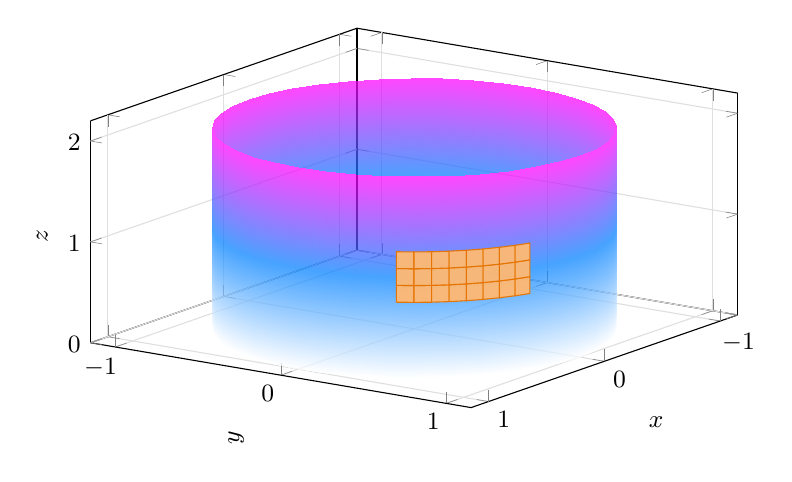
\begin{tikzpicture}
\begin{axis}[width=9.8cm,height=6.4cm,view={125}{27},axis lines=box,
    xlabel={$x$},ylabel={$y$},zlabel={$z$},
    xmin=-1.15,xmax=1.15,ymin=-1.15,ymax=1.15,zmin=0,zmax=2.2,
    xtick={-1,0,1},ytick={-1,0,1},ztick={0,1,2},
    tick label style={font=\small},label style={font=\small},
    grid=major,grid style={gray!25},domain=0:360,y domain=0:2,
    samples=41,samples y=13,z buffer=sort]
\addplot3[surf,shader=interp,colormap/cool,opacity=.72]
    ({cos(x)},{sin(x)},{y});
\addplot3[surf,shader=flat,draw=orange!90!black,fill=orange!55,
    opacity=.95,domain=30:70,y domain=.75:1.25,
    samples=9,samples y=4,z buffer=none]
    ({cos(x)},{sin(x)},{y});
\end{axis}
\end{tikzpicture}
\end{center}
\endgroup

\subsection{Orientación de una superficie}

En cada punto regular de una superficie, el plano tangente tiene una dirección perpendicular con dos sentidos opuestos. Orientar la superficie consiste en elegir uno de esos sentidos en cada punto de manera continua. Esta continuidad exige que la normal varíe sin saltos al desplazarse sobre la superficie; no se puede cambiar arbitrariamente de sentido entre parches vecinos. Si existe una elección continua en toda la superficie, se dice que esta es orientable.

La elección es relevante cuando se necesita distinguir los dos sentidos en que un campo atraviesa la superficie. Por ejemplo, para un fluido que cruza una membrana, la normal elegida permite asignar signo positivo al paso en su sentido y signo negativo al paso en el sentido contrario. Sin esta elección, el flujo con signo no queda determinado. En cambio, el área o la masa de una lámina no requieren distinguir sentidos de cruce.

Para una parametrización regular, $\vec r_u$ y $\vec r_v$ son vectores tangentes linealmente independientes. Su producto cruz es perpendicular a ambos y no es nulo. Al dividirlo entre su norma se obtiene un vector de longitud uno, sin cambiar su sentido, pues el denominador es positivo. Las dos normales unitarias locales son
\[
\mathbf n_{+}=\frac{\vec r_u\times\vec r_v}
{\lVert\vec r_u\times\vec r_v\rVert},
\qquad
\mathbf n_{-}=-\mathbf n_{+}.
\]
El sentido de $\vec r_u\times\vec r_v$ se determina mediante la regla de la mano derecha: al curvar los dedos desde $\vec r_u$ hacia $\vec r_v$ por el ángulo menor que $\pi$, el pulgar señala el sentido del producto cruz. Al invertir el orden de los factores se tiene
\[
\vec r_v\times\vec r_u=-(\vec r_u\times\vec r_v),
\]
por lo que la normal obtenida apunta en el sentido contrario. Así, el signo menos en $\mathbf n_{-}$ invierte la orientación, mientras que la normalización solo ajusta la longitud.

En una gráfica $z=f(x,y)$, con $\vec r(x,y)=\langle x,y,f(x,y)\rangle$, se obtiene
\[
\mathbf n_{+}=\frac{\langle-f_x,-f_y,1\rangle}
{\sqrt{1+f_x^2+f_y^2}},
\qquad
\mathbf n_{-}=\frac{\langle f_x,f_y,-1\rangle}
{\sqrt{1+f_x^2+f_y^2}}.
\]
La componente vertical de $\mathbf n_{+}$ es positiva, por lo que esta parametrización induce la orientación hacia arriba. Si se adopta esa orientación como positiva, $\mathbf n_{-}$ representa la negativa. Esta conclusión depende de la componente vertical, no del signo de las otras dos componentes.

En una superficie cerrada que limita un sólido, se suele adoptar como positiva la orientación exterior: la normal apunta desde el sólido hacia su exterior. Por ejemplo, en la esfera $x^2+y^2+z^2=a^2$, con $a>0$, las normales exterior e interior son
\[
\mathbf n_{\mathrm{ext}}=\frac1a\langle x,y,z\rangle,
\qquad
\mathbf n_{\mathrm{int}}=-\frac1a\langle x,y,z\rangle.
\]
La normal exterior apunta hacia arriba en el polo superior y hacia abajo en el inferior, de modo que orientación exterior y orientación hacia arriba son criterios distintos.

La figura representa las dos elecciones de normal en un mismo punto de una superficie. Ambas determinan el mismo plano tangente, pero sus sentidos son opuestos.

\begingroup\shorthandoff{>}
\begin{center}
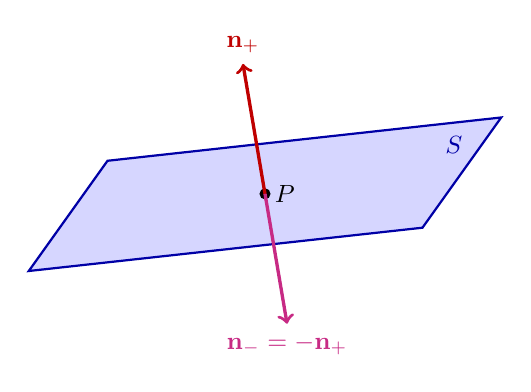
\begin{tikzpicture}[every node/.style={font=\small}]
    \fill[blue!16] (0,0)--(5,.55)--(6,1.95)--(1,1.4)--cycle;
    \draw[blue!65!black,thick] (0,0)--(5,.55)--(6,1.95)--(1,1.4)--cycle;
    \coordinate (P) at (3,.98);
    \fill (P) circle (2pt) node[right] {$P$};
    \draw[->,red!75!black,very thick] (P)--++(-.28,1.65)
        node[above] {$\mathbf n_{+}$};
    \draw[->,magenta!80!black,very thick] (P)--++(.28,-1.65)
        node[below] {$\mathbf n_{-}=-\mathbf n_{+}$};
    \node[blue!65!black] at (5.4,1.6) {$S$};
\end{tikzpicture}
\end{center}
\endgroup

La integral de un campo escalar usa $dS\geq0$ y no cambia al invertir la orientación, pues $\lVert-\vec N\rVert=\lVert\vec N\rVert$ para cualquier vector normal $\vec N$. En cambio, en el flujo interviene la componente del campo en el sentido de la normal.

\subsection{Flujo de un campo vectorial}

Sea $\mathbf F$ un campo vectorial continuo y sea $S$ una superficie orientada por una normal unitaria $\mathbf n$. En un parche pequeño de área $\Delta S$, solo la componente de $\mathbf F$ perpendicular al parche contribuye al cruce. Si $\mathbf F(P)\neq\mathbf0$, esa componente es $\mathbf F\cdot\mathbf n=\lVert\mathbf F\rVert\cos\theta$, donde $\theta$ es el ángulo entre $\mathbf F$ y la normal. La figura representa un parche $S_{ij}$, la normal elegida y un vector del campo con componente normal positiva.

\begingroup\shorthandoff{>}
\begin{center}
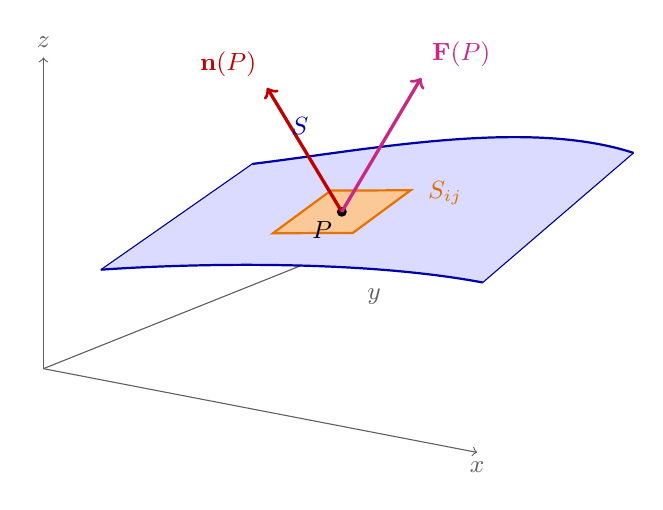
\begin{tikzpicture}[x={(1.45cm,-.28cm)},y={(1.05cm,.42cm)},z={(0cm,1.18cm)},
    every node/.style={font=\small}]
    \draw[->,gray!75!black] (0,0,0)--(3.8,0,0) node[below] {$x$};
    \draw[->,gray!75!black] (0,0,0)--(0,4,0);
    \draw[->,gray!75!black] (0,0,0)--(0,0,3.35) node[above] {$z$};
    \fill[blue!14]
        (.25,.35,1)..controls(1.2,.2,1.35)and(2.55,.35,1.65)..(3.45,.55,1.55)
        --(3.25,2.65,2.15)..controls(2.25,2.75,2.25)and(1.1,2.45,1.75)..(.2,2.25,1.45)--cycle;
    \draw[blue!65!black,thick]
        (.25,.35,1)..controls(1.2,.2,1.35)and(2.55,.35,1.65)..(3.45,.55,1.55);
    \draw[blue!65!black,thick]
        (.2,2.25,1.45)..controls(1.1,2.45,1.75)and(2.25,2.75,2.25)..(3.25,2.65,2.15);
    \draw[blue!55!black] (.25,.35,1)--(.2,2.25,1.45);
    \draw[blue!55!black] (3.45,.55,1.55)--(3.25,2.65,2.15);
    \fill[orange!45,opacity=.9]
        (1.25,1.05,1.38)--(1.95,1.05,1.55)
        --(1.95,1.75,1.76)--(1.25,1.75,1.59)--cycle;
    \draw[orange!90!black,thick]
        (1.25,1.05,1.38)--(1.95,1.05,1.55)
        --(1.95,1.75,1.76)--(1.25,1.75,1.59)--cycle;
    \coordinate (P) at (1.6,1.4,1.57);
    \fill (P) circle (1.8pt) node[below left] {$P$};
    \draw[->,red!75!black,very thick] (P)--++(-.35,-.42,1.4)
        node[above left] {$\mathbf n(P)$};
    \draw[->,magenta!80!black,very thick] (P)--++(.55,.2,1.5)
        node[above right] {$\mathbf F(P)$};
    \node[orange!85!black] at (2.25,1.75,1.8) {$S_{ij}$};
    \node[blue!65!black] at (.4,2.55,1.8) {$S$};
    \node[gray!75!black] at (0,4,-.65) {$y$};
\end{tikzpicture}
\end{center}
\endgroup

Para distinguir las componentes del campo, la siguiente figura aproxima el parche por su plano tangente en $P$ y muestra por separado las direcciones normal y tangencial.

\begingroup\shorthandoff{>}
\begin{center}
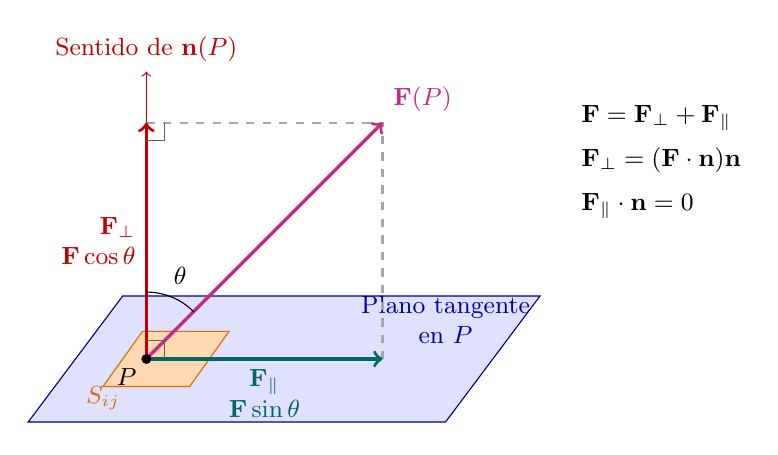
\begin{tikzpicture}[every node/.style={font=\small}]
    % El plano tangente se representa en perspectiva; la seccion
    % que contiene F y n se dibuja sin deformar sus angulos.
    \filldraw[fill=blue!12,draw=blue!55!black]
        (-1.5,-.8)--(3.8,-.8)--(5,.8)--(-.3,.8)--cycle;
    \node[blue!65!black,align=center] at (3.8,.5)
        {Plano tangente\\en $P$};
    \filldraw[fill=orange!30,draw=orange!85!black]
        (-.55,-.35)--(.55,-.35)--(1.05,.35)--(-.05,.35)--cycle;
    \coordinate (P) at (0,0);
    \coordinate (N) at (0,3);
    \coordinate (T) at (3,0);
    \coordinate (F) at (3,3);
    \draw[gray!70,dashed,thick] (N)--(F)--(T);
    \draw[->,red!75!black,very thick] (P)--(N)
        node[midway,left,align=right] {$\mathbf F_{\perp}$\\
        $\lVert\mathbf F\rVert\cos\theta$};
    \draw[->,teal!80!black,very thick] (P)--(T)
        node[midway,below,align=center] {$\mathbf F_{\parallel}$\\
        $\lVert\mathbf F\rVert\sin\theta$};
    \draw[->,magenta!80!black,very thick] (P)--(F)
        node[above right] {$\mathbf F(P)$};
    \draw[->,red!75!black] (N)--(0,3.65)
        node[above] {Sentido de $\mathbf n(P)$};
    \draw[gray!75!black] (0,.23)--(.23,.23)--(.23,0);
    \draw[gray!75!black] (0,2.77)--(.23,2.77)--(.23,3);
    \draw (0,.85) arc[start angle=90,end angle=45,radius=.85];
    \node at (.43,1.05) {$\theta$};
    \fill (P) circle (1.8pt) node[below left] {$P$};
    \node[orange!85!black] at (-.55,-.5) {$S_{ij}$};
    \node[align=left,anchor=west] at (5.4,2.5)
        {$\mathbf F=\mathbf F_{\perp}+\mathbf F_{\parallel}$\\[5pt]
        $\mathbf F_{\perp}=(\mathbf F\cdot\mathbf n)\mathbf n$\\[5pt]
        $\mathbf F_{\parallel}\cdot\mathbf n=0$};
\end{tikzpicture}
\end{center}
\endgroup

En la figura se representa el caso $0<\theta<\pi/2$. El parche se aproxima por su plano tangente en $P$, y el campo se descompone en
\[
\mathbf F_{\perp}=(\mathbf F\cdot\mathbf n)\mathbf n,
\qquad
\mathbf F_{\parallel}=\mathbf F-(\mathbf F\cdot\mathbf n)\mathbf n.
\]
Como $\mathbf n$ es unitaria, se tiene
\[
\mathbf F_{\parallel}\cdot\mathbf n
=\mathbf F\cdot\mathbf n-(\mathbf F\cdot\mathbf n)(\mathbf n\cdot\mathbf n)=0.
\]
Por tanto, $\mathbf F_{\parallel}$ pertenece al plano tangente y no tiene contribución al flujo a través del parche. La componente normal es la que atraviesa el parche y aporta el flujo aproximado
\[
(\mathbf F\cdot\mathbf n)\,\Delta S
=\lVert\mathbf F\rVert\cos\theta\,\Delta S.
\]

\begin{mydefinition}{Flujo a través de una superficie orientada}
El flujo de $\mathbf F$ a través de $S$ con la orientación $\mathbf n$ es
\[
\Phi_S(\mathbf F)=\iint_S\mathbf F\cdot\mathbf n\,dS.
\]
Un valor positivo indica cruce en el sentido de $\mathbf n$; uno negativo indica cruce en el sentido opuesto. Si $\mathbf F$ es tangente a $S$ en un punto, allí $\mathbf F\cdot\mathbf n=0$.
\end{mydefinition}

\subsubsection{Flujo a través de una gráfica}

Para $S:z=f(x,y)$ con orientación hacia arriba, la normal unitaria y el elemento de área satisfacen
\[
\mathbf n=\frac{\langle-f_x,-f_y,1\rangle}
{\sqrt{1+f_x^2+f_y^2}},
\qquad
dS=\sqrt{1+f_x^2+f_y^2}\,dA.
\]
Al multiplicar, el factor de normalización se cancela:
\[
\mathbf n\,dS=\langle-f_x,-f_y,1\rangle\,dA.
\]
\begin{mytheorem}{Flujo por una gráfica orientada hacia arriba}
Si $f$ es de clase $C^1$ sobre una región cerrada y acotada $R$, y $\mathbf F$ es continua sobre $S:z=f(x,y)$, entonces
\[
\Phi_S(\mathbf F)
=\iint_R\mathbf F\bigl(x,y,f(x,y)\bigr)
\cdot\langle-f_x(x,y),-f_y(x,y),1\rangle\,dA.
\]
Para la orientación hacia abajo, el resultado es el opuesto.
\end{mytheorem}

\paragraph{Ejemplo 5. Flujo ascendente por un paraboloide}
Sea $S:z=x^2+y^2$, $x^2+y^2\leq1$, orientada hacia arriba, y sea $\mathbf F(x,y,z)=\langle0,0,z\rangle$. Sobre $S$, el campo apunta verticalmente y su magnitud es $z=x^2+y^2$. Como $\langle-f_x,-f_y,1\rangle=\langle-2x,-2y,1\rangle$,
\begin{align*}
\Phi_S(\mathbf F)
&=\iint_R\langle0,0,x^2+y^2\rangle
\cdot\langle-2x,-2y,1\rangle\,dA\\
&=\int_0^{2\pi}\int_0^1\rho^2\,\rho\,d\rho\,d\theta
=\frac{\pi}{2}.
\end{align*}
El flujo es positivo porque el campo tiene componente en el sentido de la normal ascendente. Con orientación hacia abajo sería $-\pi/2$.

\subsubsection{Flujo a través de una superficie paramétrica}

Para $S=\vec r(D)$, el vector $\vec r_u\times\vec r_v$ es normal a la superficie. Si apunta en la orientación elegida, se tiene
\[
\mathbf n\,dS
=\frac{\vec r_u\times\vec r_v}
{\lVert\vec r_u\times\vec r_v\rVert}
\lVert\vec r_u\times\vec r_v\rVert\,du\,dv
 =(\vec r_u\times\vec r_v)\,du\,dv.
\]
De nuevo, el factor de normalización se cancela.

\begin{mytheorem}{Flujo por una superficie paramétrica}
Sea $\vec r:D\to S$ una parametrización regular que recorre $S$ una sola vez salvo, posiblemente, en la frontera. Si $\vec r_u\times\vec r_v$ apunta en la orientación elegida, entonces
\[
\Phi_S(\mathbf F)
=\iint_D\mathbf F\bigl(\vec r(u,v)\bigr)
\cdot\bigl(\vec r_u(u,v)\times\vec r_v(u,v)\bigr)\,du\,dv.
\]
Si el producto cruz apunta en sentido contrario, se cambia el signo de la integral.
\end{mytheorem}

\paragraph{Ejemplo 6. Flujo exterior por un cilindro}
En la superficie lateral del cilindro del Ejemplo 4, considérese $\mathbf F(x,y,z)=\langle x,y,0\rangle$ y la orientación exterior. Para
\[
\vec r(u,v)=\langle a\cos u,a\sin u,v\rangle
\]
se obtiene $\vec r_u\times\vec r_v=\langle a\cos u,a\sin u,0\rangle$, que apunta hacia afuera. Sobre el cilindro $\mathbf F(\vec r)=\langle a\cos u,a\sin u,0\rangle$, por lo que
\[
\Phi_S(\mathbf F)
=\int_0^{2\pi}\int_0^L a^2\,dv\,du
=2\pi a^2L.
\]
\begin{minipage}{\textwidth}
\begingroup\shorthandoff{>}
\begin{center}
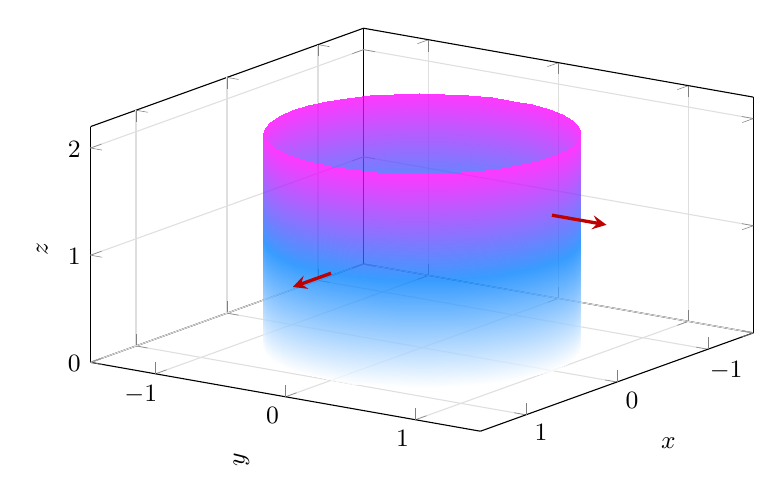
\begin{tikzpicture}
\begin{axis}[width=10cm,height=6.7cm,view={125}{27},axis lines=box,
    xlabel={$x$},ylabel={$y$},zlabel={$z$},
    xmin=-1.5,xmax=1.5,ymin=-1.5,ymax=1.5,zmin=0,zmax=2.2,
    xtick={-1,0,1},ytick={-1,0,1},ztick={0,1,2},
    tick label style={font=\small},label style={font=\small},
    grid=major,grid style={gray!25},domain=0:360,y domain=0:2,
    samples=41,samples y=13,z buffer=sort]
\addplot3[surf,shader=interp,colormap/cool,opacity=.78]
    ({cos(x)},{sin(x)},{y});
\addplot3[red!75!black,very thick,-stealth]
    coordinates {(1,0,1) (1.42,0,1)};
\addplot3[red!75!black,very thick,-stealth]
    coordinates {(0,1,1.45) (0,1.42,1.45)};
\end{axis}
\end{tikzpicture}
\end{center}
\endgroup
La figura muestra el caso $a=1$, $L=2$. Las flechas rojas indican la orientación exterior; el campo es radial y atraviesa la pared lateral en ese mismo sentido.
\end{minipage}

\subsection{Ejercicios}
\begin{enumerate}
    \setlength{\itemsep}{1pt}
    \item Evalúe $\iint_S (x+y)\,dS$ para la porción del plano $z=x+y$ situada sobre el rectángulo $0\leq x\leq1$, $0\leq y\leq2$.

    \item Evalúe $\iint_S z\,dS$ para la parte del paraboloide $z=x^2+y^2$ situada sobre el disco $x^2+y^2\leq4$.

    \item Determine la masa de la lámina $z=1+x+y$, $0\leq x,y\leq1$, si su densidad superficial es $\sigma(x,y,z)=\sigma_0(1+x)$, con $\sigma_0>0$.

    \item Determine la carga total de la esfera $x^2+y^2+z^2=a^2$ si su densidad superficial de carga es $\sigma(x,y,z)=kz$.

    \item Evalúe $\iint_S z^2\,dS$ sobre la superficie lateral del cilindro $x^2+y^2=a^2$, $0\leq z\leq L$, mediante una parametrización.

    \item Calcule el flujo de $\mathbf F=\langle0,0,1\rangle$ a través de $S:z=x^2+y^2$, $x^2+y^2\leq1$, con orientación hacia abajo.

    \item Calcule el flujo exterior de $\mathbf F=\langle x,y,z\rangle$ a través de la superficie lateral del cilindro $x^2+y^2=a^2$, $0\leq z\leq L$.

    \item Demuestre que invertir la orientación de una superficie regular conserva la integral de un campo escalar y cambia el signo del flujo de un campo vectorial.

\end{enumerate}
